%!TEX root = ../../thesis.tex
\section{Idea}

\textbf{XBMCMagic} is a web-based remote control mobile Android app for XBMC media centers\footnote{\url{http://xbmc.org}, last-checked on 21/04/2014}. Its premise is to be much more easy to use than most of the already available XBMC remote controls in the Google Play Store because makes use of gestures rather than relying on precise touch interaction.

\begin{figure}[h]
  \centerline{
    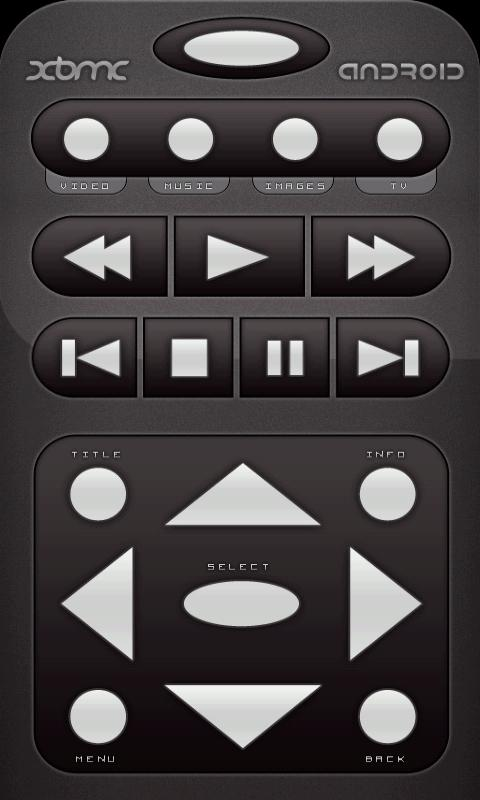
\includegraphics[width=0.4\linewidth]{images/xbmcremote.jpg}
    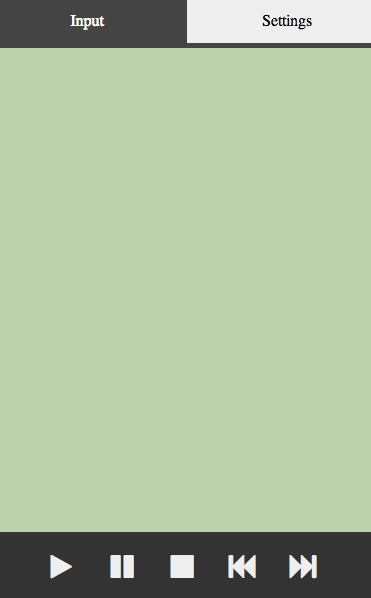
\includegraphics[width=0.414\linewidth]{images/xbmcmagic.png}
  }
  \caption[left: Official XBMC remote app, right: XBMCMagic]{left: Official XBMC remote app, right: XBMCMagic}
  \label{fig:xbmcremote}
\end{figure}

Normal remote control devices provide a haptic user interface to the user and provide tactile feedback so that they can be used blindly after some time because users can feel which are the correct buttons to use. Remote control mobile apps however rely on the device's touch interface and therefore users are not provided with a tactile feedback and they have to look at the remote control app while using it. Otherwise, they might press the wrong buttons for certain actions because the buttons are too close in the interface. \reffigure{fig:xbmcremote} shows that there are plenty of closely positioned buttons in the original XBMC remote app (left side) and the chances of picking the wrong ones are high. On the rights side of \reffigure{fig:xbmcremote}, the XBMCMagic interface is shown. It does also have buttons for basic actions such as start and stop, but the main interface is the green box above the buttons. This part of the interface detects swipe gestures and translates them into actions. The advantage of swipe gestures over buttons is that users can perform them blindly so that they do not have to look at the app when using it.